\chapter{Методика}
\label{ch:methods}

Из-за тонкой воздушной прослойки между линзой и пластиной (рис. \ref{fig:linza}), на которой она лежит, наблюдается интерференция волн. При нормальном падении света интерференционная картина наблюдается в виде концентричных колец. Если поверхность линзы содержит дефекты, то они будут наблюдаться на полученной кольцевой картине.

\begin{figure}[ht]
    \centering
    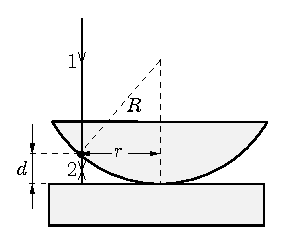
\includegraphics[width=0.3\linewidth]{./img/линза.eps}
    \caption{Оптическая схема наблюдения колец Ньютона.}
    \label{fig:linza}
\end{figure}

Геометрическая разность хода между интерферирующими лучами равна удвоенной толщине воздушного зазора $2d$ в данном месте. Для точки на сферической поверхности, находящейся на расстоянии $r$ от оси системы, имеем $r^2 = R^2 - (R - d)^2 = 2Rd - d^2$, где $R$ — радиус кривизны сферической поверхности (рис. \ref{fig:linza}).

При $R \gg d$ получим $d = r^2/2R$. С учётом изменения фазы на $\pi$ при отражении волны от оптически более плотной среды получим оптическую разность хода интерферирующих лучей:
\[
    \Delta = 2d + \frac{\lambda}{2} = \frac{r^2}{R} + \frac{\lambda}{2}.
\]

Условие интерференционного минимума $\Delta = (2m + 1)\frac{\lambda}{2}$ ($m = 0, 1, 2, \dots$), откуда получаем для радиусов тёмных колец
\[
    r_m = \sqrt{m\lambda R}.
\]

Измерив радиусы темных колец, возникающих в установке для изучения колец Ньютона при попадании на нее света с длиной волны $\lambda$, можно воспользоваться данной формулой и определить радиус кривизны линзы:
\begin{equation} \label{equ:R}
    r_m = \sqrt{m \lambda R}  \Rightarrow  R = \frac{r_m^2}{m \lambda} \ ,
\end{equation}
% где $m$ - номер темного кольца, $r_m$ - его радиус.

Из условия интерференционного минимума $\Delta = m \lambda$ с учетом $\lambda_2 < \lambda_1$ можно определить разницу длин волн $\Delta \lambda = \lambda_1 - \lambda_2$ двух спектральных компонент:
\begin{equation} \label{equ:dlamda}
    (\Delta m + 1) \lambda_2 = \Delta m \lambda_1  \Rightarrow  \Delta \lambda = \frac{\lambda_2}{\Delta m} \ ,
\end{equation}
где $\Delta m$ - количество темных колец между центрами двух четких систем.
Найти данное значение можно выделив две узкополосные спектральные компоненты из света и направив их в установку для изучения колец Ньютона, получая при этом систему колец с переменной четкостью.

В качестве источника света можно использовать ртутную лампу, излучение которой имеет определенный линейчатый спектр, и установку, содержащую исследуемую линзу для формирования колец и устройства для их наблюдения и измерения.
